\subsection{Toy example - Synthetic Dataset}
First experiments were run on synthetic data. The workflow allows to build a dataset with custom number of informative features (F), redundant features (R), copies (C) and noise (N). Redundant features are our main aim, and they depend on F features, usually their squared version. The generated values are random and the target is build using only items $\in$ F.

After swapping, the results show:

\begin{itemize}
    \item Features $\in$ F are not related to each other in the diagram, therefore discriminations performs well.
    \item Copied features behave as expected, since they hold a strong (mutual) relation to their informative features. Again, copies are not related among them.
    \item Redundant features consistent in terms of relation, i.e. they are related to their Original feature’ copies, and other redundants. E.g. R02 to F02, C02 and Cos02.
\end{itemize}

\begin{figure}[!h]
	\centering
	\begin{subfigure}[b]{0.3\linewidth}
		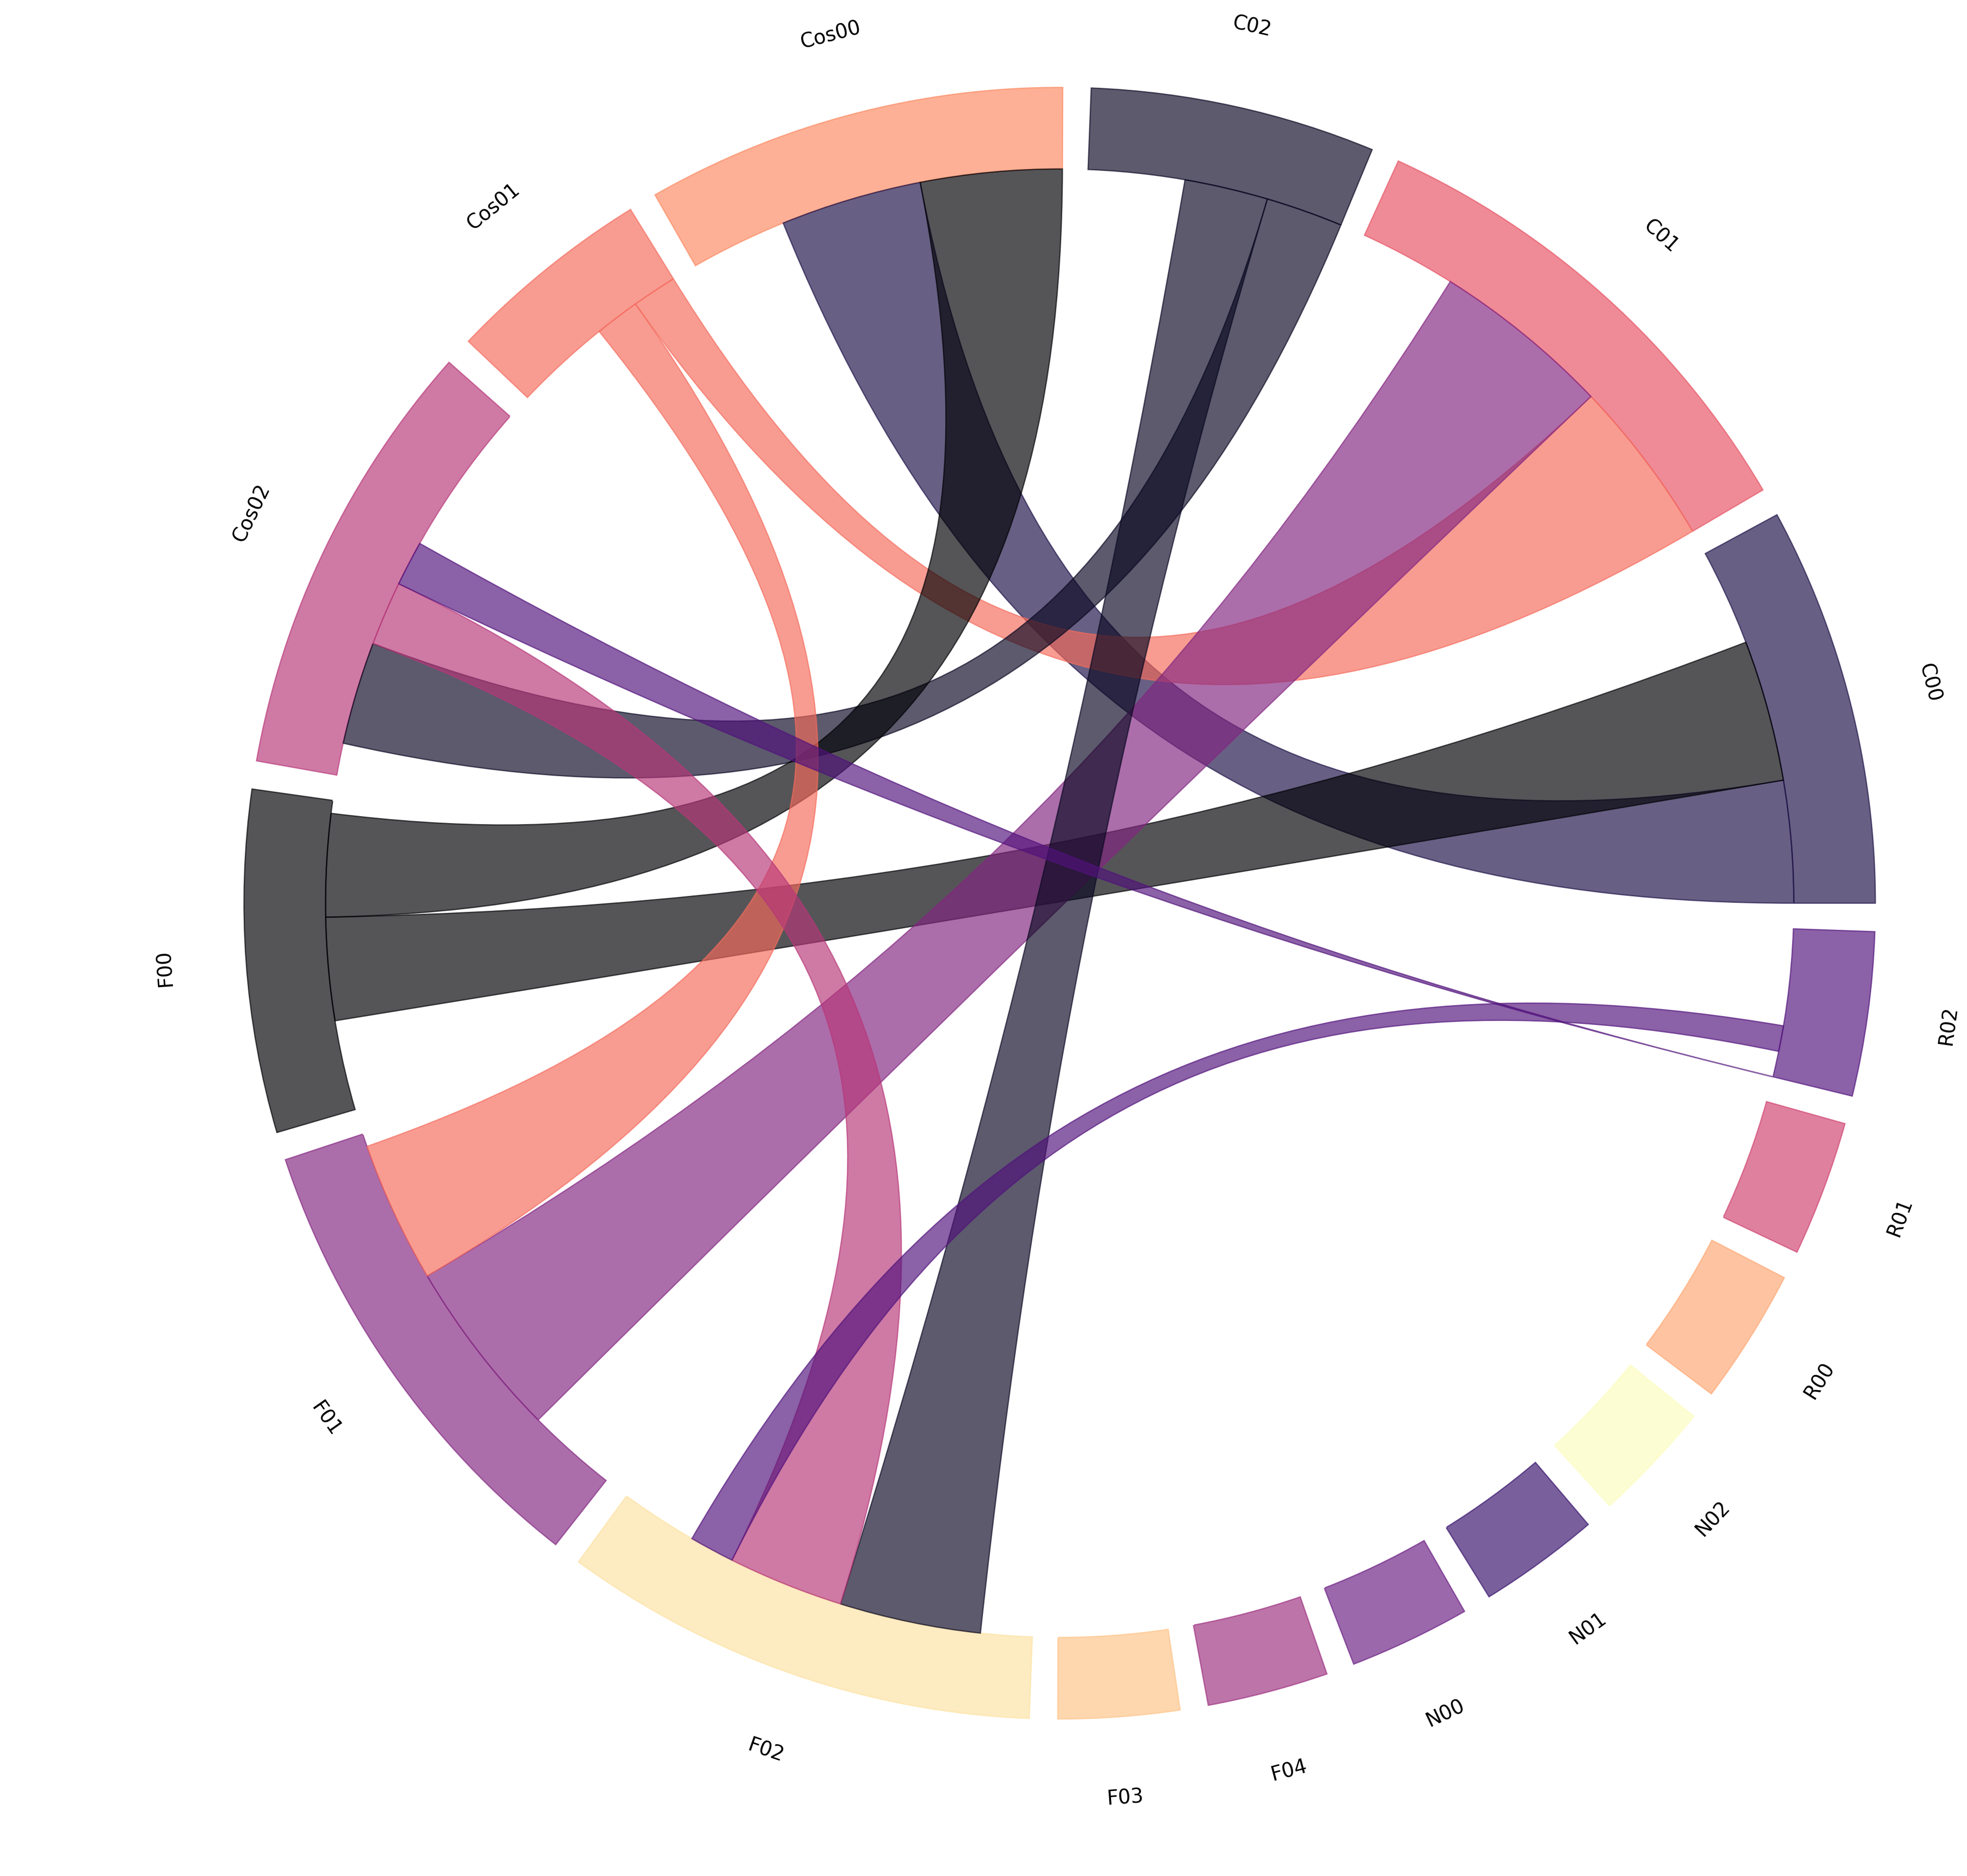
\includegraphics[width=\linewidth]{figures/chords/chord_swap_ensemble1000_RCN5333300_097.png}
		\caption{Chord diagram representation at \emph{t} = 0.98}
	\end{subfigure}
	\hfill
	\begin{subfigure}[b]{0.3\linewidth}
		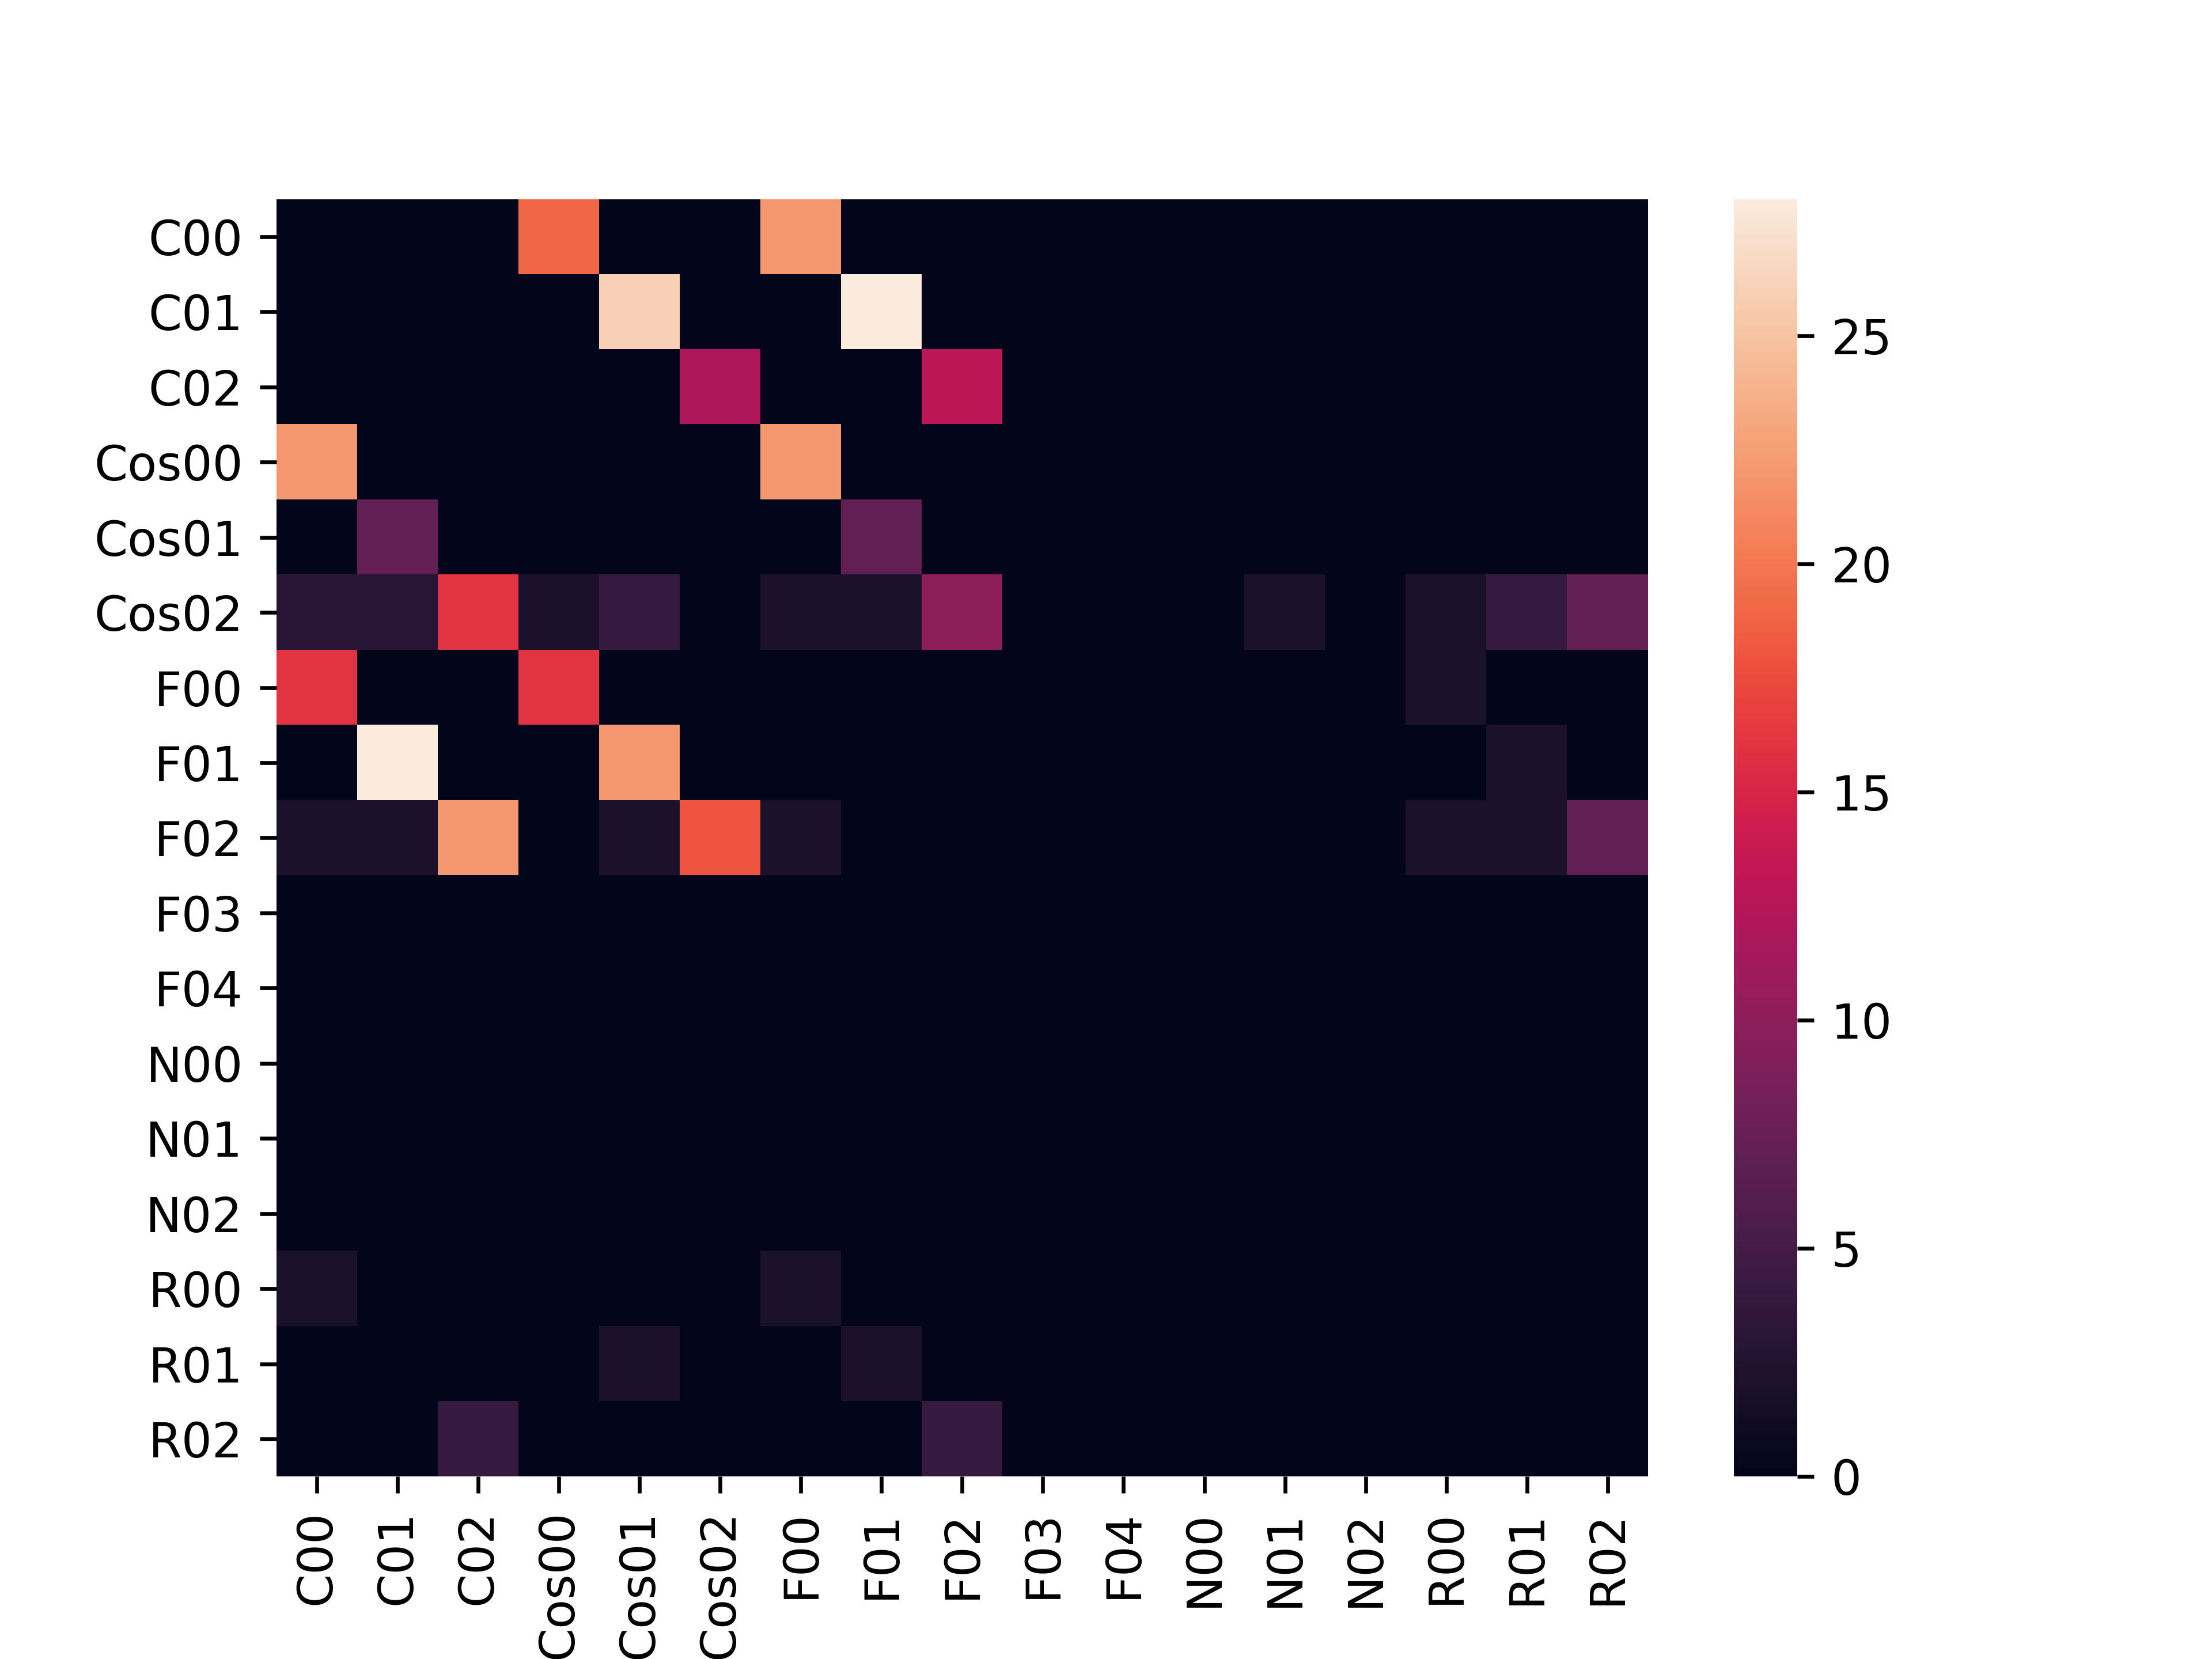
\includegraphics[width=\linewidth]{figures/heatmaps/heatmap_swap_ensemble1000_RCN5333300_097.png}
		\caption{Heatmap from matrix at \emph{t} = 0.98. Edge thickness indicates relation strength.}
	\end{subfigure}
	\hfill
	\begin{subfigure}[b]{0.3\linewidth}
		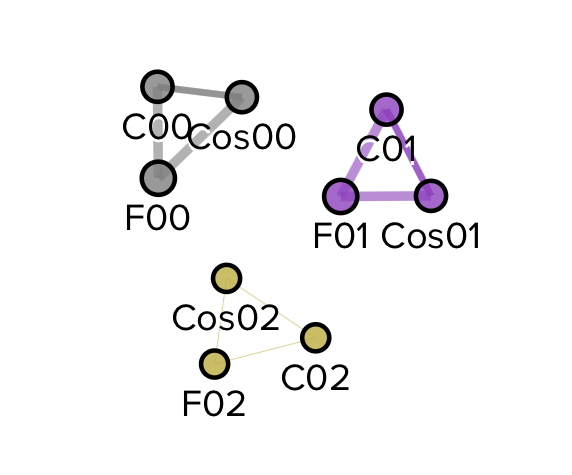
\includegraphics[width=\linewidth]{Major Thesis/figures/graphs/graph-toy.png}
		\caption{Graph clustering at \emph{t} = 0.98}
	\end{subfigure}
	\label{fig:triade}
	\caption{Clustering process. (a) Shows relation in Chord diagram to ease visualisation. (b) Gives the matrix which we post-process to keep only relevant links. (c) Final relation graph. Each connected component is a final group whose representative is the most connected node. Community detection algorithms colour each group.}
\end{figure}

On the other hand, we also found a drawback: Some redundant features relate to other than theirs. E.g R00 relates to F01, F02. However, the relation is stronger to R00, which can only by filtered by a threshold modification, allowing only relations above 0.97 get past it. Evolution of the relations using a moving threshold can be found in Suppl. Material \ref{suppl:relations}

\subsubsection{Gain/Loss summary}
Accuracy may vary along the swapping method, hence can also derive an overview of the general tendency as shown in Figure \ref{fig:gainloss}. The difference score is calculated by substracting the new accuracy (using the new swapped set) to the old one (original set). If the result is positive, we tag it as \emph{gain}, and otherwise as \emph{loss}. If the scores are exactly the same, we use \emph{equal}.

\begin{figure}[!h]
	\centering
	\captionsetup{justification=centering}
	\begin{subfigure}[b]{0.45\linewidth}
		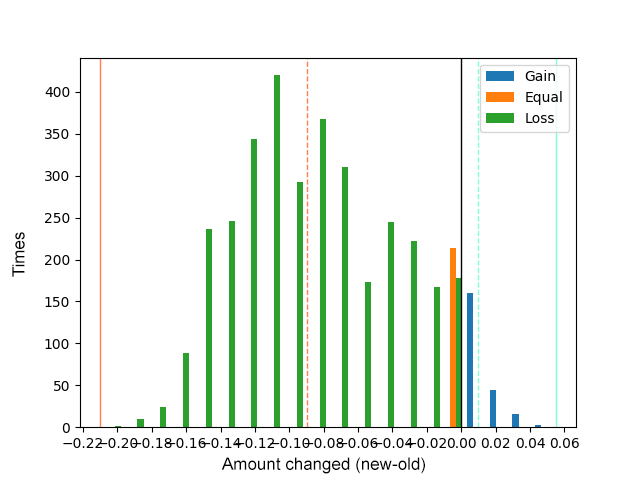
\includegraphics[width=\linewidth]{Major Thesis/figures/gain_loss/swap_ensemble1000_RCN5333300.png}
		\caption{1000 samples (RCN) 5 Inf, 3 Red, 3 Copy, 3 Cosine, 3 Noise}
	\end{subfigure}
	\hfill
	\begin{subfigure}[b]{0.45\linewidth}
		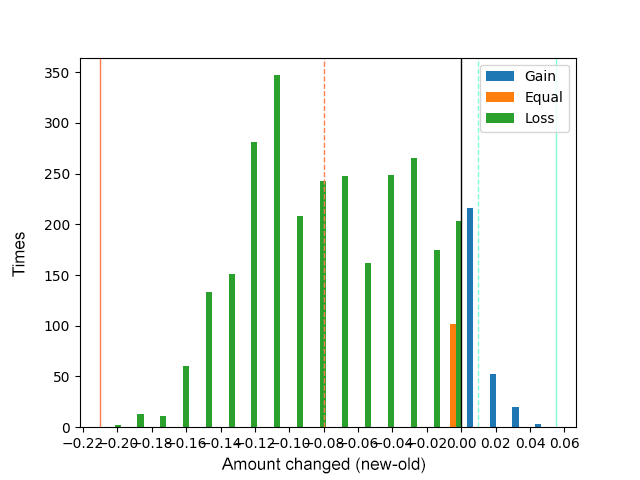
\includegraphics[width=\linewidth]{Major Thesis/figures/gain_loss/swap_ensemble1000_RN5053200.png}
		\caption{1000 samples (RN) 5 Inf, 0 Copy, 5 Red., 3 Cosine, 2 Noise}
	\end{subfigure}
	\caption{Gain/Loss summary on synthetic data. Full lines on each side indicate the maximum value for each group (Gain or Loss). Dashed lines compute the median of the group. The middle line tags the 0 value for reference purposes.}
	\label{fig:gainloss}
\end{figure}

\subsection{Diabetes Type 2 - Real Dataset}
Using a SNP dataset can deliver confusing results. Features which are detected as redundant can be swapped/grouped to obtain the same result. 

Normalised scores show the following pattern: When plotting the graph step by step (one threshold increase in descending sorted order), the variables added tend to have 0.95 Jaccard similarity in the original data. Besides, for each addition, we add a node to the connected component and do not form new ones. If any CC is created, it is soon linked.
\\

Not-normalised scores show the same pattern, except the node additions is more exponential, i.e. it does not add one node at the time but several.
Testing the similarity score among features by randomly picking them shows a bimodal distribution: either the results are close to 0.9 or to 0.1, which mich be causing the bias in the swapper.

\begin{figure}[!hp]
	\centering
	\captionsetup{justification=centering}
	\begin{subfigure}[b]{0.45\linewidth}
		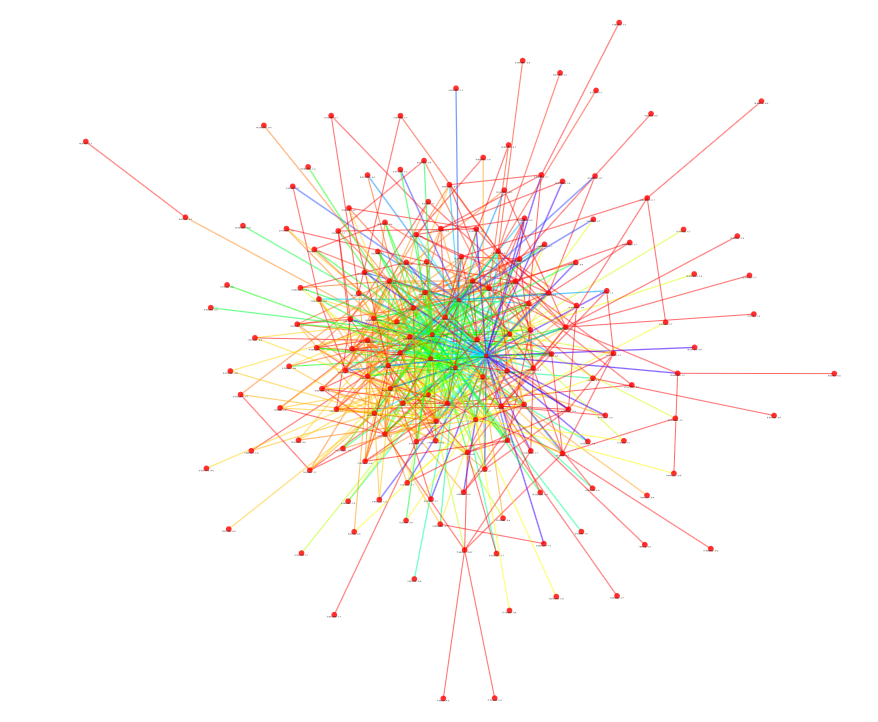
\includegraphics[width=\linewidth]{Major Thesis/figures/graphs/dt2_ssc0.2_0.8ssc.png}
		\caption{All nodes included.}
	\end{subfigure}
	\hfill
	\begin{subfigure}[b]{0.45\linewidth}
		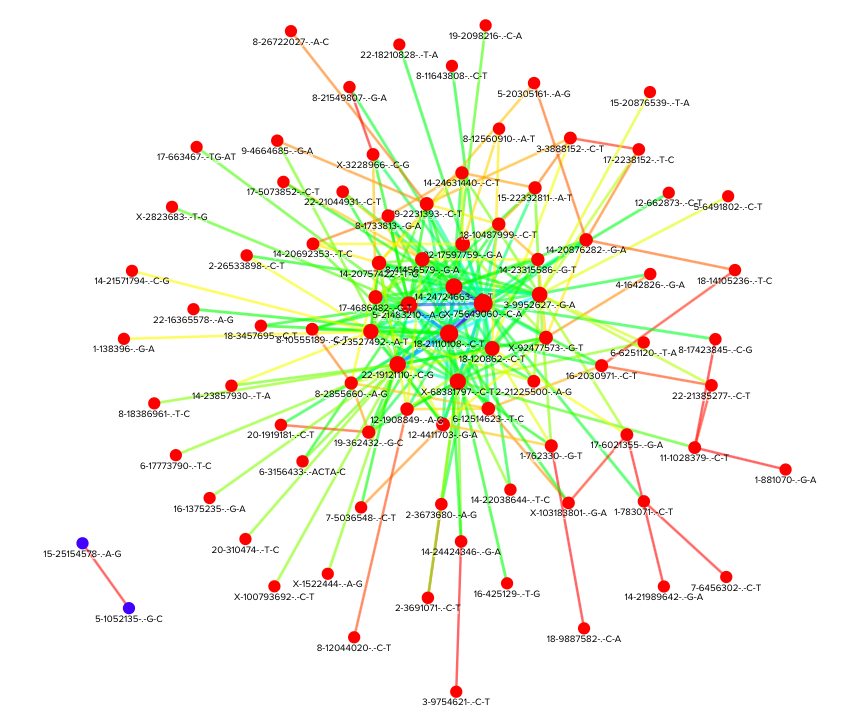
\includegraphics[width=\linewidth]{Major Thesis/figures/graphs/dt2_ssc0.2_0.8ssc_mean.png}
		\caption{Scores above mean.}
	\end{subfigure}
	\caption{Relations among variables after full swapping top \emph{ensemble} variables with all feature set. Results filtered at WRS\footnote{WRS = Weak Relevance Score}=1, JSC\footnote{Jaccard Similarity Score}<0.2 and 0.8>JSC.}
    \label{fig:dt2-trimmed}
\end{figure}

\subsubsection{Time complexity}